\documentclass[class=scrreprt]{standalone}

\usepackage{amssymb}
\usepackage{amsmath}
\usepackage{pgfplots}
\pgfplotsset{compat=newest}
\pgfplotsset{hide scale/.style={
/pgfplots/xtick scale label code/.code={},
/pgfplots/ytick scale label code/.code={}}}
\usepgfplotslibrary{groupplots}

\KOMAoptions{fontsize=9pt}


\begin{document}

\begin{tikzpicture}[]
	
\definecolor{color_m2}{RGB}{100,175,25}
         
\begin{scope}[xshift = 0cm, yshift = 0cm]
	\begin{axis}[
			at={(1cm,1cm)},
			width=4cm,
			height=4cm,
			scale only axis=true,
			axis lines = left,
			hide scale,
			xmin=0,
			xmax=5e6,
			xtick={0,1e6,2e6,3e6, 4e6, 5e6},
			xticklabels={,,,,},
			scaled x ticks = false,
			ymin=-0.005,
			ymax=0,
			ytick={-.005, -0.0025, 0},
			yticklabels={,,},
			yminorgrids=false,
			xmajorgrids=true,
			ymajorgrids=true,
			legend style={fill=white, fill opacity=0, draw opacity=1, text opacity=1,draw=none}, 
			legend pos=south west,
			legend cell align={left}
		]
		  
		\addplot[color=olive, solid, thick] 
		table[x =n, y=c] {Fracture anisotropy maximization/Results_compression/f_Tcomp_compression.txt};
		
		\addplot[color=black, solid, thick] 
		table[x =n, y=c] {Fracture anisotropy maximization/Results_compression/f_Trand_compression.txt};
		
		\addplot[color=color_m2, dotted, thick] 
		table[x =n, y=c] {Fracture anisotropy maximization/Results_compression/f_Tae_compression.txt};
		
		\addplot[color=color_m2, solid, thick] 
		table[x =n, y=c] {Fracture anisotropy maximization/Results_compression/f_Tpost_compression.txt};
	\end{axis}
	
	\node[black] at (0.25,4.75) {\textbf{A}};
	\node[black,right] at (0.9,0.75) {\noexpand\noexpand\noexpand\footnotesize{$0\cdot 10^{6}$}};
	\node[black,left] at (5.1,0.75) {\noexpand\noexpand\noexpand\footnotesize{$5\cdot 10^{6}$}};
	\node[black] at (3,0.5) {$n_F$};
	
	\node[black,right,rotate=90] at (0.75,0.9) {\noexpand\noexpand\noexpand\footnotesize{$-5\cdot 10^{-3}$}};
	\node[black,left, rotate=90] at (0.75,5.1) {\noexpand\noexpand\noexpand\footnotesize{$0\cdot 10^{-3}$}};
	\node[black, rotate=90] at (0.4,3) {$\min(J_{\text{comp}})$};
	 
	 
	% Add the designs
	\begin{scope}[xshift=1.1cm, yshift=2.65cm]
	\filldraw[white] (0,0) rectangle(1.5,1.5); 
	\node[] at (0.75,0.75) {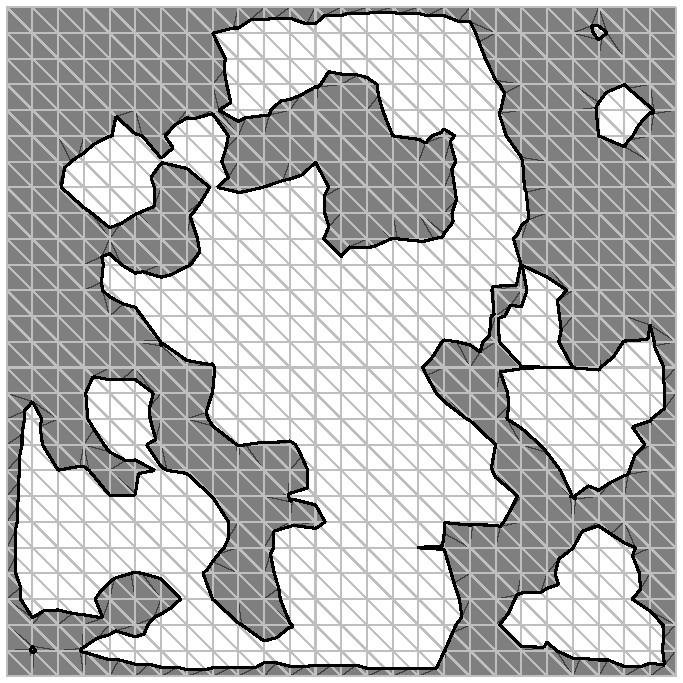
\includegraphics[width=1.5cm]{Fracture anisotropy maximization/Results_compression/Design_rand_compression.pdf}};
	\draw[black, thick] (0,0) rectangle(1.5,1.5);
	\end{scope}
	         
	\begin{scope}[xshift=2.65cm, yshift=1.1cm]
	 \filldraw[white] (0,0) rectangle(1.5,1.5);
	 \node[] at (0.75,0.75) {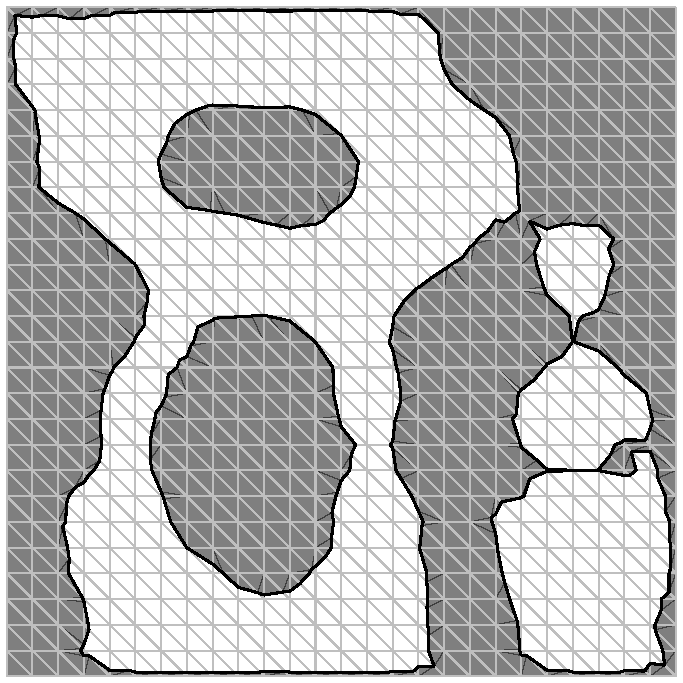
\includegraphics[width=1.5cm]{Fracture anisotropy maximization/Results_compression/Design_post_compression.pdf}};
	\draw[color_m2, thick] (0,0) rectangle(1.5,1.5);
	\end{scope}
\end{scope}

\begin{scope}[xshift = 5cm, yshift = 0cm]
	\begin{axis}[
			at={(1cm,1cm)},
			width=4cm,
			height=4cm,
			scale only axis=true,
			axis lines = left,
			hide scale,
			xmin=0,
			xmax=5e6,
			xtick={0,1e6,2e6,3e6, 4e6, 5e6},
			xticklabels={,,,,},
			scaled x ticks = false,
			ymin=-0.005,
			ymax=0,
			ytick={-.005, -0.0025, 0},
			yticklabels={,,},
			yminorgrids=false,
			xmajorgrids=true,
			ymajorgrids=true,
			legend style={fill=white, fill opacity=0, draw opacity=1, text opacity=1,draw=none}, 
			legend pos=south west,
			legend cell align={left}
		]
		  
		\addplot[color=olive, solid, thick] 
		table[x =n, y=c] {Fracture anisotropy maximization/Results_compression/f_Tcomp_compression.txt};
		
		\addplot[color=black, solid, thick] 
		table[x =n, y=c] {Fracture anisotropy maximization/Results_expansion/f_Trand_expansion.txt};
		
		\addplot[color=color_m2, dotted, thick] 
		table[x =n, y=c] {Fracture anisotropy maximization/Results_expansion/f_Tae_expansion.txt};
		
		\addplot[color=color_m2, solid, thick] 
		table[x =n, y=c] {Fracture anisotropy maximization/Results_expansion/f_Tpost_expansion.txt};
	\end{axis}
	
	\node[black] at (0.25,4.75) {\textbf{B}};
	\node[black,right] at (0.9,0.75) {\noexpand\noexpand\noexpand\footnotesize{$0\cdot 10^{6}$}};
	\node[black,left] at (5.1,0.75) {\noexpand\noexpand\noexpand\footnotesize{$5\cdot 10^{6}$}};
	\node[black] at (3,0.5) {$n_F$};
	
	\node[black,right,rotate=90] at (0.75,0.9) {\noexpand\noexpand\noexpand\footnotesize{$-5\cdot 10^{-3}$}};
	\node[black,left, rotate=90] at (0.75,5.1) {\noexpand\noexpand\noexpand\footnotesize{$0\cdot 10^{-3}$}};
	\node[black, rotate=90] at (0.4,3) {$\min(J_{\text{exp}})$};
	 
	 
	% Add the designs
	\begin{scope}[xshift=1.1cm, yshift=2.65cm]
	\filldraw[white] (0,0) rectangle(1.5,1.5); 
	\node[] at (0.75,0.75) {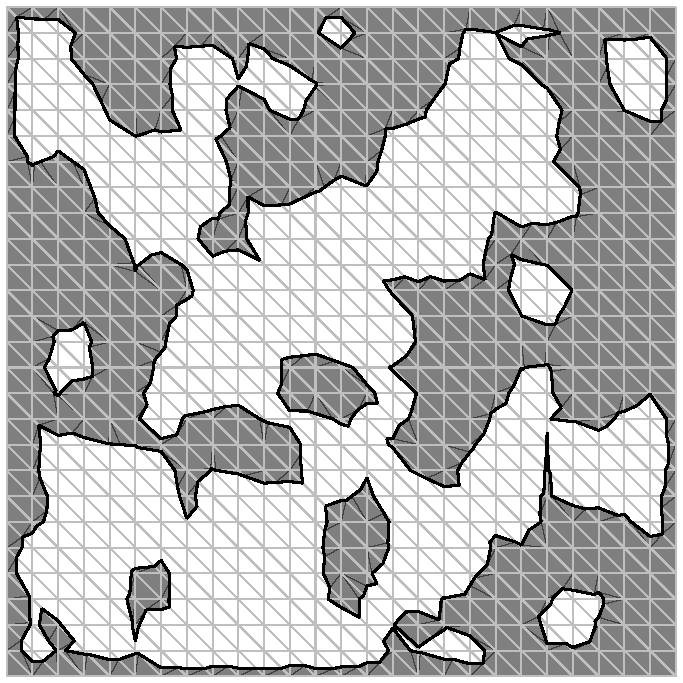
\includegraphics[width=1.5cm]{Fracture anisotropy maximization/Results_expansion/Design_rand_expansion.pdf}};
	\draw[black, thick] (0,0) rectangle(1.5,1.5);
	\end{scope}
	         
	\begin{scope}[xshift=2.65cm, yshift=1.1cm]
	 \filldraw[white] (0,0) rectangle(1.5,1.5);
	 \node[] at (0.75,0.75) {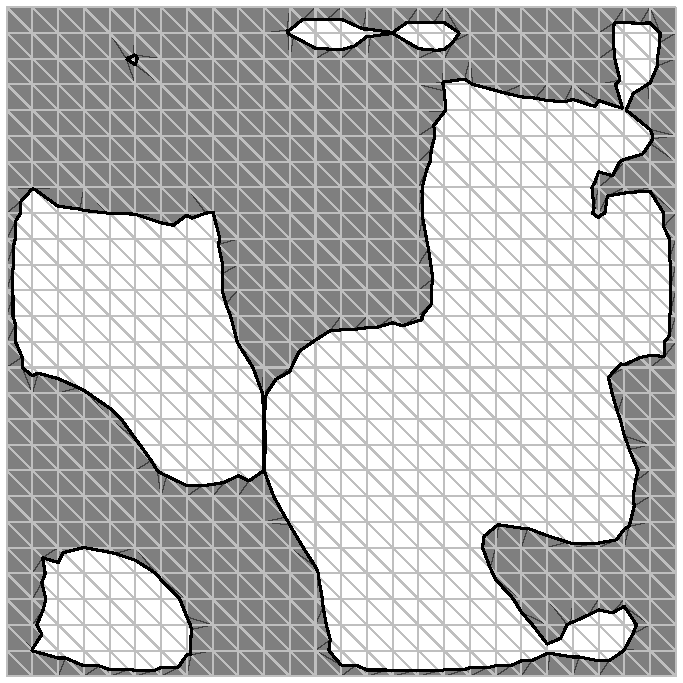
\includegraphics[width=1.5cm]{Fracture anisotropy maximization/Results_expansion/Design_post_expansion.pdf}};
	\draw[color_m2, thick] (0,0) rectangle(1.5,1.5);
	\end{scope}
\end{scope}

\begin{scope}[xshift = 10cm, yshift = 0cm]
	\begin{axis}[
			at={(1cm,1cm)},
			width=4cm,
			height=4cm,
			scale only axis=true,
			axis lines = left,
			hide scale,
			xmin=0,
			xmax=5e6,
			xtick={0,1e6,2e6,3e6, 4e6, 5e6},
			xticklabels={,,,,},
			scaled x ticks = false,
			ymin=-10e-3,
			ymax=0,
			ytick={-10e-3, -5e-3, -0e-3},
			yticklabels={,,},
			yminorgrids=false,
			xmajorgrids=true,
			ymajorgrids=true,
			legend style={fill=white, fill opacity=0, draw opacity=1, text opacity=1,draw=none}, 
			legend pos=south west,
			legend cell align={left}
		]
		  
		\addplot[color=olive, solid, thick] 
		table[x =n, y=c] {Fracture anisotropy maximization/Results_compression/f_Tcomp_compression.txt};
		
		\addplot[color=black, solid, thick] 
		table[x =n, y=c] {Fracture anisotropy maximization/Results_shear/f_Trand_shear_adj.txt};
		
		
		\addplot[color=color_m2, dotted, thick] 
		table[x =n, y=c] {Fracture anisotropy maximization/Results_shear/f_Tae_shear_adj.txt};
		
		\addplot[color=color_m2, solid, thick] 
		table[x =n, y=c] {Fracture anisotropy maximization/Results_shear/f_Tpost_shear_adj.txt};
	\end{axis}
	
	\node[black] at (0.25,4.75) {\textbf{C}};
	\node[black,right] at (0.9,0.75) {\noexpand\noexpand\noexpand\footnotesize{$0\cdot 10^{6}$}};
	\node[black,left] at (5.1,0.75) {\noexpand\noexpand\noexpand\footnotesize{$5\cdot 10^{6}$}};
	\node[black] at (3,0.5) {$n_F$};
	
	\node[black,right,rotate=90] at (0.75,0.9) {\noexpand\noexpand\noexpand\footnotesize{$-1\cdot 10^{-16}$}};
	\node[black,left, rotate=90] at (0.75,5.1) {\noexpand\noexpand\noexpand\footnotesize{$0\cdot 10^{-16}$}};
	\node[black, rotate=90] at (0.4,3) {$\min(J_{\text{shear}})$};
	 
	 
	% Add the designs
	\begin{scope}[xshift=1.1cm, yshift=1.1cm]
	\filldraw[white] (0,0) rectangle(1.5,1.5); 
	\node[] at (0.75,0.75) {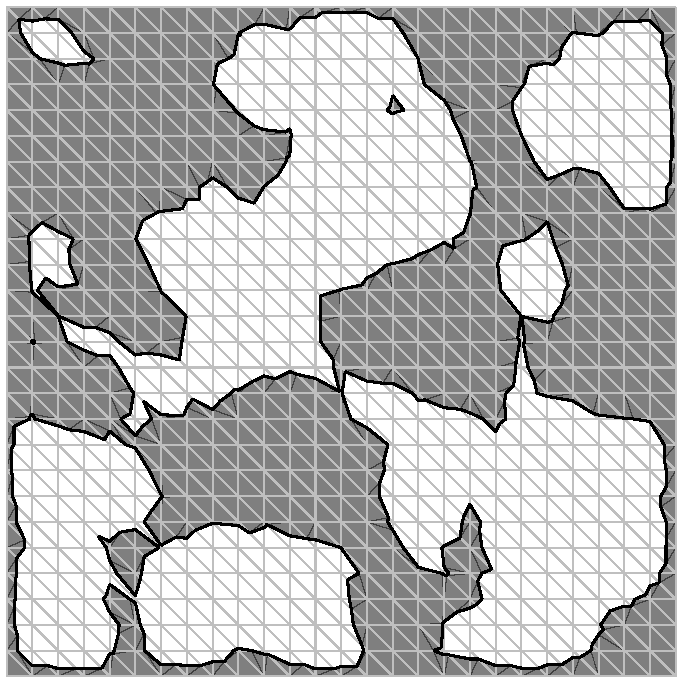
\includegraphics[width=1.5cm]{Fracture anisotropy maximization/Results_shear/Design_rand_shear.pdf}};
	\draw[black, thick] (0,0) rectangle(1.5,1.5);
	\end{scope}
	         
	\begin{scope}[xshift=3.4cm, yshift=2.65cm]
	 \filldraw[white] (0,0) rectangle(1.5,1.5);
	 \node[] at (0.75,0.75) {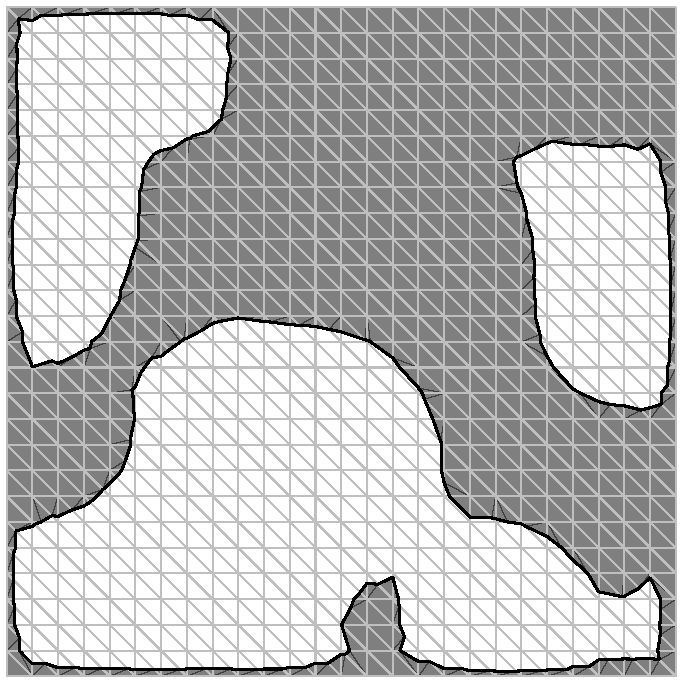
\includegraphics[width=1.5cm]{Fracture anisotropy maximization/Results_shear/Design_post_shear.pdf}};
	\draw[color_m2, thick] (0,0) rectangle(1.5,1.5);
	\end{scope}
\end{scope}
         
                
         
        

\filldraw[draw=black,fill=black!20!white] (1,-0.75) rectangle (15,0);
        \begin{axis}[
            at = {(1cm,-0.75cm)},
            axis lines = left,
            axis line style={draw=none},
            width=14cm,
            height=0.75cm,
	    scale only axis=true,
            enlargelimits=false,
            xlabel = ,
            ylabel = ,
            xmajorgrids=true,
	    ymajorgrids=true,
    	    legend columns = 3,
            legend style={fill=none, draw=none,  at={(0,0.5)}, anchor=west, style={column sep=0.175cm}},
            legend cell align=center,
            xmin=0,
            xmax=0.1,
            xtick={\empty},
            ymin=0,
            ymax=0.1,
            ytick={\empty},
        ]
        
         \addplot[ 
                 color=olive,
                 solid,thick,
             ] coordinates {(1,1) (2,1)};

             \addplot[ 
                 color=black,
                 solid,thick,
             ] coordinates {(1,1) (2,1)};
             
             \addplot[ 
                 color=color_m2,
                 solid,thick,
             ] coordinates {(1,1) (2,1)};


        
        
        
        \legend{{$DE_{300,300,0.6,0.9}$, $\mu = 50$}, {Training samples}, {Proposed method, $m=50$}};

        \end{axis}

 \end{tikzpicture}
 \end{document}